\section{Понятие неявно заданной функции.
Существование, непрерывность и дифференцируемость неявно заданной функции,
системы неявно заданных функций.}

\subsection{Понятие неявно заданной функции от одной переменной}Предположим, что значения двух переменных $x$ и $y$ связаны между собой уравнением, которое в общем случае имеет вид

\begin{equation}\label{def1}
    F(x, y) = 0
\end{equation}

Тогда функция $y = f(x)$ называется \emph{неявной}, если она задана при посредстве \emph{неразрешённого} относительно $y$ уравнения~(\ref{def1})

\subsection{Теорема о существовании и дифференцируемости неявно заданной функции}

\subsubsection*{Формулировка}

Пусть 
\begin{enumerate}
    \item функция $F(x, y)$ непрерывна и имеет в окрестности точки $M_0(x_0, y_0)$
    непрерывные частные производные
    \item $F(x_0, y_0) = 0$
    \item $F'_y(x_0, y_0) \neq 0$
\end{enumerate}
Тогда
\begin{enumerate}
    \item в некоторой окрестности 
    \begin{equation*}
        \mathfrak{D}_0 = (x_0 - \delta, x_0 + \delta; y_0 - \delta', y_0 + \delta')
    \end{equation*}
    точки $M_0 (x_0, y_0)$ уравнение~(\ref{def1}) определяет $y$ как однозначную
    функцию от $x$: $y = f(x)$;
    \item $f(x_0) = y_0$
    \item в проемежутке $(x_0 - \delta, x_0 + \delta)$ функция $f(x)$ непрерывна и
    \item она имеет в этом промежутке непрерывную производную
\end{enumerate}

\subsubsection*{Доказательство}

\begin{enumerate}
    \item Пусть, без ограничения общности, $F'_y(x_0, y_0) > 0$. В силу непрерывности 
    производной $F'_y$, она будет положительна и в достаточно малой окрестности точки 
    $(x_0, y_0)$ (например в такой, где выполняется неравенство 
    $|F'_(x,y) - F'(x_0, y_0)| < F'_y(x_0, y_0)$). Возьмём замкнутый прямоугольник
    \begin{equation*}
        \mathfrak{D} = [x_0 - \delta', x_0 + \delta'; y_0 - \delta', y_0 + \delta']
    \end{equation*}
    целиком лежащий в этой окрестности, так что написанное неравенство имеет место во всех
    его точках.\\
    Отсюда сразу вытекает, что --- при любом постоянном $x$ из промежутка $[x_0 - \delta', x_0 + \delta']$ --- $F(x, y)$ как функция от $y$ будет монотонно возрастающей.\\
    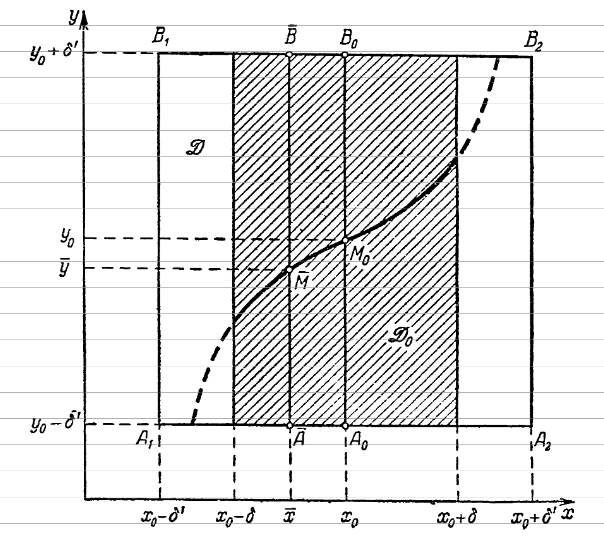
\includegraphics[width=2.5in]{30rect.png}\\
    Станем двигаться вдоль вертикали, проходящей через точку $M_0$, т.е. фиксируем $x = x_0$,тогда рассматриваемая функция $F(x, y)$ сведётся к функции $F(x_0, y)$ от одной переменной. В силу второго условия, при $y = y_0$ она обращается в ноль. В тоже время как мы сейчас установили функция возрастает вместе с $y$, так что для $y < y_0$ её значение меньше нуля, а для $y > y_0$ --- больше. В частности, следовательно, она будет иметь значения разных знаков в точках $A_0(x_), y - \delta')$ и $B_0(x_0, y + \delta')$.\\
    Перейдём теперь к горизонтальным прямым, проходящим через эти точки, т.е. зафиксируем $ y = y_0 + \delta'$ и $y = y_0 - \delta'$. Получатся две функции от одной переменной $F(x, y_0 + \delta')$ и $F(x, y_0 - \delta')$, которые при $x = x_0$ имеют разные знаки. Но по условию 1) эти функции непрерывны, т.е. найдётся некоторая окрестность $(x_) - \delta, x_0 + \delta)$, в которой обе функции сохраняют свой знак, так что при $x_0 -\delta < x < x_0 + \delta$
    \begin{equation*}
        F(x, y_0 - \delta') < 0, F(x, y_0 + \delta')
    \end{equation*}
    Иными словами, на нижнем и верхнем основаниях $A_1A_2$ и $B_1B_2$ исходного прямоугольника вдоль отрезков длины $2\delta$ с центрами в точках $A_0$ и $B_0$ заданная функция имеет отрицательные значения на первом и положительные на втором. Фиксируем в промежутке $(x_0 - \delta, x_0 + \delta)$ любое значение $x = \bar{x}$ и рассмотрим вертикальный отрезок, соединяющий точки $\bar{A}(\bar{x}, y_0 - \delta')$ и $\bar{B}(\bar{x}, y_0, + \delta')$. Вдоль него наша функция снова сведется к функции $F(\bar{x}, y)$ от одной переменной. О ней мы знаем, что
    \begin{equation*}
        F(\bar{A}) < 0, F(\bar{B}) > 0
    \end{equation*}
    Тогда по теореме Больцано-Коши, при некотором значении $y = \bar{y}$, содержащемся между $y_0 - \delta'$ и $y_0 + \delta'$, эта функция обращается в ноль: 
    \begin{equation*}
        F(\bar{x}, \bar{y}) = 0
    \end{equation*}
    Из монотонности следует, что при  $y \geq \bar{y}$ функция будет не меньше нуля, так что $\bar{y}$ есть единственное значение $y$ в промежутке $(y_0 - \delta', y_0 + \delta')$, которое совместно с $x = \bar{x}$ удовлетворяет уравнению~(\ref{def1}).\\
    Таким образом в окрестности
    \begin{equation*}
        \mathfrak{D}_0 = [x_0 - \delta, x_0 + \delta; y_0 - \delta', y_0 + \delta']
    \end{equation*}
    точки $M_0$ уравнение~(\ref{def1}) действительно определяет $y$ как однозначную функцию от $x$: $y = f(x)$
    \item Утверждение 2) прямо следует из доказательства предыдущего пункта, $y_0$ и есть тот единственный $y$, при котором $F(x_0, y_0) = 0$;
    \item Придадим $x$ приращение $\Delta x$, ему будет соответствовать единственное значение \\$y + \Delta y = f(x + \Delta x)$ вместе с ним удовлетворяющее уравнению~(\ref{def1}). Очевидно и приращение 
    \begin{equation*}
        \Delta F(x, y) = F(x + \Delta x, y + \Delta y) - F(x, y)= 0
    \end{equation*}
    Преобразуем теперь это выржение, используя формулу конечных приращений (теорему Лагранжа):
    \begin{equation*}
        0 = F(x + \Delta x, y + \Delta y) - F(x, y) = |F(x + \Delta x, y + \Delta y) - F(x, y + \Delta y)| +
    \end{equation*}
    \begin{equation*}
        + |F(x, y + \Delta y) - F(x, y)| = F'_x(x + \theta \Delta x, y + \Delta )\cdot \Delta x + F'_y(x, y + \theta_1 \Delta y)\cdot\Delta y
    \end{equation*}
    \begin{equation*}
        (0 < \theta, \theta_1 < 1)
    \end{equation*}
    откуда
    \begin{equation}\label{eq2}
        \frac{\Delta y}{\Delta x} = - \frac{F'_x(x + \theta \Delta x, y + \Delta )}{F'_y(x, y + \theta_1 \Delta y)}
    \end{equation}
    Но непрерывная в $\mathfrak{D}$ функция $|F'_x|$ ограничена сверху конечным числом $M$ (по теореме Кантора):
    \begin{equation*}
        |F'_x| \leq M
    \end{equation*}
    и в то же время положательная непрерывная функция $F'_y$, иемющая в $\mathfrak{D}$ наименьшее значение $m$, также положительное, ограничена им снизу:
    \begin{equation*}
        F'_y \geq m > 0
    \end{equation*}
    Отсюда
    \begin{equation*}
        \left| \frac{\Delta y}{\Delta x} \right| \leq \frac{M}{m} \implies |\Delta y| \leq \frac{M}{m}|\Delta x|
    \end{equation*}
    А отсюда напрямую следует утверждеие 3
    \item Возвращаясь к равенству~(\ref{eq2}), предположим теперь, что $\Delta x \rightarrow 0$. Так ка мы уже знаем, что при этом и $\Delta y \rightarrow 0$ то, по непрерывности частных производных и с учётом того, что $F'_y \neq 0$, справа в пределе получим
    \begin{equation*}
        - \frac{F'_x(x, y)}{F'_y(x, y)}
    \end{equation*}
    Таков же будет и предел левой части равнства~(\ref{eq2}), так что существует производная $y$ по $x$:
    \begin{equation*}
        f'(x) = y'_x = \lim_{\Delta x \to 0}\frac{\Delta y}{\Delta x} = - \frac{F'_x(x, y)}{F'_y(x, y)}
    \end{equation*}
    отсюда очевидно, что $f'(x)$ --- также непрерывная функция
\end{enumerate}

\subsection{Неявная функция от нескольких переменных}

Аналогично уравнению~(\ref{def1}), можно рассматривать и уравнение с большим числом переменных. Пусть, например, имеем уравнение с тремя переменными:
\begin{equation}\label{def3}
    F(x, y, z) = 0
\end{equation}
При известных условиях $z$ определяется как неявная функция от двух переменных $x$ и $y$

\subsection{Определение нявных функций из системы уравнений}

В самом общем случае нам может быть даан система из $m$ уравнений с $n + m$ переменными:
\begin{equation}\label{eq4}
    \left.
    \begin{array}{c}
        F_1(x_1, \dots, x_n; y_1, \dots, y_m) = 0,\\
        F_2(x_1, \dots, x_n; y_1, \dots, y_m) = 0,\\
        \dots\\
        \dots\\
        F_m(x_1, \dots, x_n; y_1, \dots, y_m) = 0,\\
    \end{array}
    \right\}
\end{equation}
Здесь речь идёт об определении этой системой $m$ переменных $y_1, \dots, y_m$, как неявных функций от $n$ переменных $x_1, \dots, x_n$:
\begin{equation*}
    y_1 = f_1(x_1, \dots, x_n), \dots, y_m = f_m(x_1, \dots, x_n)
\end{equation*}
так, что при подстановке их в~(\ref{def3}) получаются тождества относительно $x_1, \dots, x_n$
